\chapter{Theoretische Grundlagen}
\label{chap:two}
In diesem Kapitel wird der theoretische Rahmen für die weiteren Kapitel gelegt. Im
ersten Abschnitt werden die Grundlagen der bibliothekarischen Statistik im Zusammenhang mit Budgetplanung
und Mittelallokation erläutert. Der darauf folgende Abschnitt handelt von Datenvisualisierungen und deren Einsatz
für Datenrepräsentationen. Abschließend wird das Modell der Business-Intelligence-Software als Schmelzpunkt der 
beiden vorangegangen Kapitel eingeführt.

\section{Bibliothek und Statistik}
\label{chap:two_one}
% Bibliotheksrahmen - Etatplanung - Etatbedarfe, Zielsetzung der Bibliothek
Die Etatplanungen von Bibliotheken richten sich nach deren Informations- und Versorgungsauftrag. 
Seit Beginn der 1990er Jahre kämpfen Bibliotheken mit dem größer werdenden Informationsangebot, den steigenden Preisen auf dem Publikationsmarkt, 
den zunehmenden Kommerzialisierungstendenzen in der Verlagslandschaft und den neuen Medientypen. 
Zu nennen wären hier konkret: die Explosion der Zeitschriftenpreise im Bereich der \acrfull{STM}, die Konzentration auf wenige Verlage, 
das Aufkommen von Ebooks. Demgegenüber steigen Bibliotheksetats nur mäßig. 
Somit geht ein Kaufkraftverlust einher \cite[Vgl.][161]{moravetz-kuhlmann_monika_erwerbungspolitik_2015}.
Diese Entwicklung betrifft nicht nur Universitätsbibliotheken, sondern auch Spezialbibliotheken von Forschungseinrichtungen.
Bibliotheken haben Instrumente entwickelt, um den Informationsauftrag trotz dieser Widrigkeiten zu erfüllen.
Es entstehen von Bund und Ländern geförderte Konsortien, um den Kostendruck auf Bibliotheken im Bereich der elektronischen
Fachinformationen zu mildern. Neue Geschäftsmodelle wurden dies bezüglich entwickelt, um Preisnachlässe bei den Verlagen zu erzielen
\cite[Vgl.][169 ff.]{moravetz-kuhlmann_monika_erwerbungspolitik_2015}. Das Projekt \textit{Deal} - ein Projekt der Hochschulrektorenkonferenz (HRK) in Zusammenarbeit mit den
wissenschaftlichen Einrichtungen in Deutschland - konnte so in den vergangenen Jahren Verträge mit den Verlagen Springer oder Wiley erfolgreich abschließen \cite[Vgl.][]{projekt_deal_projekt_2020}.

Um den Veränderungen des Publikationsmarktes lokal in der Bibliothek zu begegnen, wird es immer wichtiger, das Bibliotheksbudget und die Mittelallokation kosteneffizient zu planen. 
Dies geschieht bisher in größeren Bibliotheken durch Etatbedarfs- und Etatverteilungsmodelle, die sich seit den 1990er Jahre etablierten.(Quelle) 
%Ziel dieser Modelle ist die effiziente Mittelallokation 
% transparente und gerechte Verteilung knapper Ressourcen% innerhalb der Bibliothek. 
% Mittelallokation bezeichnet die Verteilung knapper Ressourcen. 
Diese Modelle basieren auf der Erhebung von bibliothekarischen Kennzahlen \cite[Vgl.][172 ff.]{moravetz-kuhlmann_monika_erwerbungspolitik_2015}

%Was ist Statistik\\
%hat schon immer große Rolle in Bibliotheken gespielt\\
%BIX, Deutsche Bibliotheksstatistik (seit wann)\\
Bibliotheksstatistik reflektiert das Gestern, Heute und Morgen, indem 
sie die bibliothekarischen Servicedienstleistungen evaluiert und den Zielen und Aufgaben anpasst \cites[Vgl.][2 f.]{jilovsky_cathie_library_2004}[Vgl.][462]{laitinen_markku_library_2013}.
Im deutschen Bibliothekswesen gibt es die umfangreiche \acrfull{DBS}. 
Träger der \textit{\acrshort{DBS}} sind das \acrfull{hbz NRW},  das \acrfull{KBN}, \acrfull{KMK} sowie die Bibliotheken.
Aufgabe der \textit{\acrshort{DBS}} ist die jährliche Erhebung der Statistikdaten von Kennzahlen von Bibliotheken. 
Seit 1999 werden die Daten nur noch online erfasst, ausgewertet und präsentiert \cite[Vgl.][2]{schmidt_deutsche_2008}.
Neben den Gesamtauswertungen der DBS, einer Bibliothekssuchmachine für Öffentliche Bibliotheken, 
bietet sie eine variable Auswertung nach individuellen Abfragen der DBS-Daten. 
Dennoch ist die \textit{\acrshort{DBS}} vielmehr eine Datengrundlage für die Auswertung der Daten als eine Auswertung solcher.
Daneben gab es den \acrfull{BIX}, der ursprünglich für die Leistungsmessung in Öffentlichen Bibliotheken konzipiert wurde. 
2002 wurde er erweitert auf das Wissenschaftliche Bibliothekssystem. Der \textit{\acrshort{BIX}} wurde 2015 aufgrund von Finanzierungsproblemen eingestellt. 

%Erhebung von qualitativen und quantitativen Daten Bsp.:\\
Bibliothekarische Kennzahlen werden durch quantitative und qualitative Evaluationsverfahren des Bestandes erhoben.
Bestand ist nach Johannsen und Mittermaier \textit{„... die Gesamtheit aller Medien, die eine Bibliothek ihren Nutzern anbietet, sei es, dass sie diese 
„physisch“ besitzt, sei es, dass sie entsprechende Nutzungsrechte erworben hat.“} \cite[252]{johannsen_jochen_bestands-_2015}.
Als Typen der Bestandsevaluation sind sammlungs-, nutzungsbezogene und nutzerbezogene Evaluationen zu nennen.\cite[Vgl.][302]{johnson_peggy_fundamentals_2014}
Basieren die sammlungs- und nutzungsbezogene Evaluation auf quantitativen Daten, greift die nutzer:innenbezogene Evaluation zu meist auf qualitative Daten zurück. 
\cite[Vgl.][461 ff.]{blake_data_2004}.

Die sammlungsbezogene Evaluation betrifft die Größe des Bestandes und das Wachstum über die Jahre. Die Bestimmung der Bestandsstärke- und tiefe, 
der Ausgewogenheit in den Bestandssegmenten sind Ziele der sammlungsbezogenen Evaluation. 
Ebenfalls lässt sich die Frage nach der aktuellsten Literatur im Bestand oder in einem Segment durch die sammlungsbezogene Evaluation klären.

Nutzungsbezogene Evaluation umfasst die Lesesaalnutzung, die Ausleihe vor-Ort, die Nutzung des Fernleihservices oder Dokumentenlieferdienste und die Online-Nutzung von elektronischen Ressourcen \cite[Vgl.][254 ff.]{johannsen_jochen_bestands-_2015}.
Die Frage nach den Zugriffsstatistiken von elektronischen Ressourcen beansprucht darin einen immer größer werdenden Raum.
Die internationale Organisation \acrfull{COUNTER} gibt dazu die COUNTER-Statistiken heraus. Mitglieder der Organisation sind Verlage, Bibliotheken
und Zwischenhändler. Die COUNTER-Statistiken sind mittlerweile der Quasi-Standard für die Zugriffsstatistiken 
auf elektronischer Ressourcen geworden. Diese werden getrennt nach Art der Informationsressourcen in verschiedenen Reports herausgegeben. \cite[Vgl.][260 ff.]{johannsen_jochen_bestands-_2015}. 
Mittlerweile ist die fünfte Iteration der COUNTER-Statistiken \textit{\acrshort{COP 5}} erschienen \cite{counter_abstract_2020}.
%Im Jahr 2019 ersetzte sie die vorhergehende Version.
Die Bibliotheken sind dabei auf die Unterstützung der Verlage angewiesen. Diese stellen unregelmäßig diese \textit{\acrshort{COP 5}}-Statistiken zur
Verfügung. Ziele der nutzungsbezogenen Evaluation sind die Identifizierung von ausleihträchtigen Medienbeständen (Vormerkungs- und Rennerlisten), 
die Deacquisition schlecht oder gar nicht genutzter Titel. Ebenso kann die Evaluation von Fernleih- und Dokumentenlieferungen Hinweise auf Bestandslücken liefern
\cite[Vgl.][255 ff.]{johannsen_jochen_bestands-_2015}. Als Konsequenz aus den COUNTER-Statistiken kann die Abbestellung von elektronischen Ressourcen resultieren.

Die nutzer:innenbezogene Evaluation ist auf den Nutzer:innenkreis und dessen Informationsbedürfnisse zentriert. 
%Fundamental ist der Unterschied zwischen den einzelnen Evaulationsverfahren in der Erhebung der Daten. 
Die sammlungs- und nutzungsorientierten Evaluationsverfahren basieren auf der Erhebung von quantitativen Daten wie Bestandsgröße oder der Anzahl von Ausleihen nach Titel. 
Während nutzerbezogene Evaluation qualitative Daten, die aus Befragungen erhebt.
%Warum ist Messbarkeit von bibliothekarischen Daten wichtig?\\
%Welchen Impact für Budgetplanung können statistische Daten haben?\\

Die einzelnen Evalualtionen vermitteln ein realistisches Gesamtbild der Bibliothek und deren Service-Dienstleistungen. 
Die datengetriebenen Evalutionsauswertungen bieten Hinweise auf Optimierungen der bibliothekarischen Service-Dienstleistungen. 
Die Auswertungen können durch die Bibliotheksleitung aufgenommen werden und in strategische (zukünftigen) Entscheidungen miteinfliessen. 
So kann ein detailliertes Erwerbungsprofil und somit eine gezieltere Erwerbungspolitik entstehen. 
Dadurch wird das Management der Ressourcen zudem effektiver und effizienter \cite[Vgl.][297]{johnson_peggy_fundamentals_2014}.
Gegenüber Stakeholdern kann auf der Grundlage der Evaluationen gezielt um Budget verhandelt werden.
\textit{„The purpose of the statistics is to give the management of the library or another decision-maker 
a satisfactory and correct picture about the situation of the library as a support to them - the statistics are the mirror of the library!”}
\cite[463]{laitinen_markku_library_2013}
Um ein zufriedenstellendes und korrektes Bild der Situation der Bibliothek zu präsentieren, können sorgsam ausgewählte Datenvisualisierungen helfen.

\section{Datenvisualisierung}
Datenvisualisierung ist der Zucker auf den Daten.
Der Begriff der Datenvisualisierung umschreibt die visuelle Repräsentation und Präsentation von Daten \cite[Vgl.][15]{kirk_data_2019}.
%Oberbegriff für Informationsvisualisierung / Scientific Visualization\\
Er wird in Teilen der Literatur als Oberbegriff für „Information visualization” oder „Scientific Visualization” verstanden \cite[Vgl.][11]{few_now_2009}.
% Abgrenzung zu Infographics
Datenvisualisierung grenzt sich in Form und Inhalt von Infografiken ab. 

Infografiken haben die Aufgabe Nachrichten zu kommunizieren.
Sie bestehen aus einem Mix von Diagrammen, Karten, Illustrationen und Text. Klarheit und Tiefe der Darstellungen sind dabei wichtig
\cite[Vgl.][31]{cairo_truthful_2016}. Sie werden auch als „Explanation Graphics”
bezeichnet und bestimmen sich dadurch, dass sie Geschehen und Ereignisse graphisch erzählen. 
Historisch sind Infografiken mit dem Medium der Printzeitungen und Printzeitschriften verbunden \cite[Vgl.][27]{kirk_data_2019}.

% Was ist unter Datenvisualisierung zu verstehen?\\
Datenvisualisierung hingegen ist eine Anzeige von Daten, die Analyse, Exploration und Entdeckung ermöglichen soll.
Sie sind nicht primär dafür gemacht Geschichten über die Informationen zu erzählen. Sie dienen als Werkzeug, um aus den visualisierten Daten Schlussfolgerungen zu ziehen 
\cite[Vgl.][31]{cairo_truthful_2016}.


Es finden sich in der Literatur verschiedene Eigenschaften von Datenvisualisierungen.
Datenvisualisierungen basieren auf gründlicher und ernsthafter Forschung. Sie sind funktional, dass heißt
sie bemühen sich die Daten genau darzustellen. Darüber hinaus sind Datenvisualisierungen attraktiv, 
aufschlussreich und erhellend \cite[Vgl.][45]{cairo_truthful_2016}. 
Ferner sollen Datenvisualisierungen computerunterstützt und interaktiv sein \cite[Vgl.][12]{few_now_2009}.


Datenvisualisierungen arbeitet mit visuellen Elementen wie Graphen, Diagrammen, Tabellen und Karten.
Mit dem Einsatz dieser visuellen Elemente sollen Muster, Trends und Ausnahmen in Daten leichter sichtbar gemacht werden\cite[Vgl.][12]{few_now_2009}.
Datenvisualisierungen setzen einen visuellen Reiz, der schneller vom menschlichen Auge verarbeitet werden kann. 
Deswegen sind mit dem Einsatz der visuellen Elemente Muster, Trends und Ausnahmen in den Daten leichter erkennbar.
% Zweck der Datendarstllung Bindung an Daten
Um Muster, Trends und Ausnahmen bei größer werdenden Datenmengen zu erkennen, reichen Tabellen aber nicht mehr aus. Deswegen
kommen andere visuelle Elemente wie Diagramme zum Einsatz. 


Im Vorfeld einer Datenvisualisierung ist zu überlegen, wie die Beschaffenheit der Daten ist und welcher Zweck durch die Datenvisualisierung erreicht werden soll.
% Wie sind die Daten skaliert. Nominalskalen Ordinalskala, Verhältnisskalen, diskrete Werte oder kontinuierliche Werte
Diese Überlegungen bestimmen die Verwendung der visuellen Elemente. 
Welche Merkmale und Eigenschaften sollen durch die Visualisierung gezeigt werden.\cite[Vgl.][17]{kirk_data_2019}
% Verwendung von Zeitreihen -> Linecharts Ausleihen über die Jahre lassen sich mit Liniencharts darstellen ...
% Welchen Zweck sollen Daten erfüllen -> wem gegenüber soll etwas kommuniziert werden

Mit den Siegeszug des Computers in den 1980/90er Jahren sind \dots\\
leicht verschiedene Begriffsdefinitionen
Vielzahl von Begriffen\\ 
Zu welchem Zweck\\
Eigenschaften\\
Wie Datenvisualisierungen gestaltet werden sollen - simpel\\
Grundlage - Daten - quantitativ / qualitativ
Warum Datenvisualisierung wichtig ist?\\
Was erzählen Datenvisualisierungen mehr als Zahlenkolonnen?\\
Welche Datenvisualisierungen gibt es?\\
Wo kommen Daternvisualisierungen zum Einsatz?\\

Um sich einen Überblick zu verschaffen welche Daten in einem Unternehmen anfallens, kann man diese auf einen Dashboard sammeln.
Dashboards sind Intanzen von Business-Intelligence-Software.


% \begin{figure}[ht]
%     \centering
%         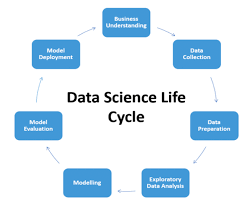
\includegraphics[width=8cm]{ds_cycle}
%         \caption{Data Science Cycle}
%         \label{fig:data science}
% \end{figure}



\clearpage
\section{Business-Intelligence-Systeme}

Was sind Business-Intelligence-Löungen?\\
%Wo kommen Buisiness-Intelligence-Lösungen zum Einsatz zum Einsatz?
Es gibt eine Vielzahl kommerzieller Lösungen für den Bibliotheksbereich, die auf Business-Intelligence-Software basieren.
Zu nennen wären \textit{AlmaAnalytics} für das Next-Generation-Library-System \textit{Alma} von \textit{ExLibris}\footnote{\url{https://www.exlibrisgroup.com/products/alma-library-services-platform/alma-analytics}
Stand: 26.05.2020}, \textit{BibControl} von \textit{OCLC}\footnote{\url{https://www.oclc.org/de/bibcontrol.html} Stand: 26.05.2020},
\textit{CollectionHq} von \textit{Baker \& Taylor}\footnote{\url{https://www.collectionhq.com/} Stand: 26.05.2020} oder \textit{Libinsight} von \textit{SpringShare}\footnote{\url{https://springshare.com/libinsight/} Stand: 26.05.2020}.
Darüber hinaus gibt es Business-Intelligence-Applikationen, die von
Bibliotheken für Reporting, Datenanalyse und Datenvisualisierung adaptiert werden,
wie zum Beispiel \textit{Tableau} von der Firma \textit{Tableau Software} oder
\textit{Crystal Reports} von \textit{SAP}.
Diese Applikationen sind entweder
an bestimmte Bibliothekssysteme zurückgebunden, limitiert in ihren
Funktionen\cite{golas_statistische_2018} oder zu generisch.
Überdies wird sowohl von \textit{HeBis} bzw. von der
Lokal-Bibliothekssystembetreuung als auch von der \textit{mpdl} keine Applikation
in dieser Richtung angeboten.
Ebenso ist ungewiss, wann die Ablösung des schon betagten \textit{CBS/LBS} hin zu
einem neuen Next-Generation-Library-System im \textit{HeBis-Verbund} stattfinden wird und ob
es ein Modul zur statistischen Datenerhebung liefern wird.
